\documentclass{IEEEtran4PSCC}

% packages
\usepackage{lipsum}
\usepackage{ulem}
\usepackage{hyperref}
% \usepackage{flushend}
\usepackage[inline]{enumitem}
\usepackage{array,multirow,graphicx}
\usepackage{float}
\usepackage{orcidlink}

%% footnote
\usepackage{footnote}
\makesavenoteenv{tabular}
\makesavenoteenv{table}
\makesavenoteenv{tabular*}
\makesavenoteenv{table*}
% \usepackage{tablefootnote}

%% graphics packages
\usepackage{tikz}
\usepackage{colortbl}
\usepackage{pgfplots}
\usepackage{graphicx}
\usepackage{multirow}
\usepackage{multicol}
\usepackage{circuitikz}
\usepackage{dblfloatfix}
\usepackage[bottom]{footmisc}
\ifCLASSOPTIONcompsoc
    \usepackage[caption=false, font=normalsize, labelfont=sf, textfont=sf]{subfig}
\else
    \usepackage[caption=false, font=footnotesize]{subfig}
\fi

%% checkmark packages 
\usepackage{pifont}
\newcommand{\cmark}{\ding{51}}
\newcommand{\xmark}{\ding{55}}

%% math packages
\usepackage{amssymb}
\usepackage[cmex10]{amsmath}
\usepackage{mathtools}
\usepackage{booktabs}

% math 
\IEEEeqnarraydefcolsep{0}{\hoffset}
\newcommand*{\defeq}{\stackrel{\text{def}}{=}}

% definition setup
%\theoremstyle{definition}

\newtheorem{defn}{Definition}[section]

% correct bad hyphenation here
\hyphenation{op-tical net-works semi-conduc-tor}

% Set footer
\makeatletter
\let\old@ps@headings\ps@headings
\let\old@ps@IEEEtitlepagestyle\ps@IEEEtitlepagestyle
\def\psccfooter#1{%
    \def\ps@headings{%
        \old@ps@headings%
        \def\@oddfoot{\strut\hfill#1\hfill\strut}%
        \def\@evenfoot{\strut\hfill#1\hfill\strut}%
    }%
    \def\ps@IEEEtitlepagestyle{%
        \old@ps@IEEEtitlepagestyle%
        \def\@oddfoot{\strut\hfill#1\hfill\strut}%
        \def\@evenfoot{\strut\hfill#1\hfill\strut}%
    }%
    \ps@headings%
}
\makeatother

\psccfooter{%
        \parbox{\textwidth}{\hrulefill \\ \small{24th Power Systems Computation Conference} \hfill \begin{minipage}{0.2\textwidth}\centering \vspace*{4pt} 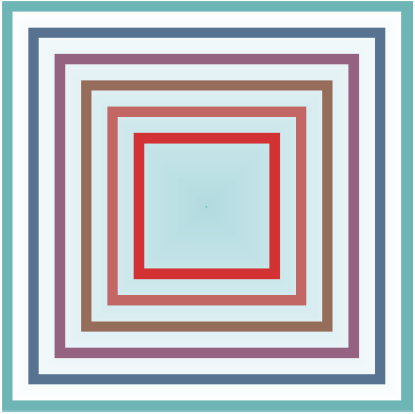
\includegraphics[scale=0.06]{PSCC_logo.png}\\\small{PSCC 2026} \end{minipage} \hfill \small{Limassol, Cyprus --- June 8 -- June 12, 2026}}%
}

\begin{document}

\onecolumn
\title{ Efficient Uncertainty Quantification of Cable Parameters using Linear Error Propagation and Chaos Polynomial Methods}

\author{ 
\IEEEauthorblockN{ Amauri G. Martins Britto\orcidlink{0000-0002-2691-9061}, Tom Van Acker\orcidlink{0000-0001-6283-1457}, Hakan Ergun\orcidlink{0000-0001-5171-1986}, and Ruth V. Sabariego\orcidlink{0000-0001-7515-3923} }
\IEEEauthorblockA{\textit{Department of Electrical Engineering} \\
\textit{KU Leuven \& the Etch Competence Hub of EnergyVille} \\
Leuven / Genk, Belgium\\ }}

\maketitle

\vspace{-.5cm}{\it Index terms} -- Cable parameters, polynomial chaos expansion, transmission line theory, uncertainty quantification.\thanksto{\noindent This work is supported by the Energy Transition Fund by FOD Economy, Belgium, project HARMONIC. The General Board on Energy of the FOD Economy is not liable for any use of the presented work and subsequent results.}

\section{Motivation}
The increasing integration of renewable energy sources has resulted in a greater reliance on complex underground and sub-marine cable systems, which present significant modeling challenges compared to traditional overhead lines \cite{Karmokar2025}. The per-unit-length impedances (Z) and admittances (Y) of cable systems are influenced by mutual couplings in intricate geometries and material properties, and are subject to uncertainties arising from manufacturing tolerances, installation conditions, e.g., burial depth and proximity to other cables, and ambient characteristics, e.g., soil resistivity. Consequently, the rigorous quantification of variability in these Z and Y parameters has gained increasing research attention, driven by its direct influence on critical power system studies including fault and protection analysis, transient behavior assessment, and harmonic hosting capacity \cite{tom_van_acker_impact_2025}.

\section{Novel Contributions}
This research provides a comprehensive benchmark of different methods for uncertainty quantification of frequency-dependent Z- and Y-parameters of complex power system cables, including: Linear Error Propagation (LEP), Polynomial Chaos Expansion (PCE) and Monte Carlo (MC) simulation. The comparative analysis yields critical insights into how inherent physical model non-linearities influence the propagation of uncertainties. Moreover, the study establishes the practical value of PCE for generating complete stochastic representations and performing parametric sensitivity assessments for these physically realistic, frequency-dependent cable systems, advancing beyond common simplifications reported in the existing literature \cite{Manfredi2020, Triverio2015}.

\section{The Proposed Approach}
An open-source analytical framework \cite{amauri_g_martins_britto_linecablemodelsjl_nodate}, which provides frequency-dependent Z and Y matrices for multi-layer power cables with inherent LEP, serves as the deterministic model. Physical input uncertainties, e.g., layer thicknesses and material electromagnetic properties, are defined as random variables reflecting typical manufacturing and operational variabilities. Three uncertainty quantification (UQ) techniques are systematically compared using the framework, namely: Linear Error Propagation, Polynomial Chaos Expansion and Monte Carlo. The resulting statistical moments and distributions of the output frequency-dependent R, L, and C parameters are analyzed to assess accuracy, computational burden, and to quantify model non-linearities, followed by a PCE-based parametric sensitivity analysis.

\section{Numerical Experiments and Validation}
A multi-layer coaxial cable system based on actual design data is defined as the primary test case. A high-fidelity ground truth model is established using Finite Element Method (FEM). Next, the proposed toolbox is employed for its native LEP implementation, and as the engine for PCE and extensive MC simulations. Output R, L, C statistics and sensitivities from LEP, MC, and PCE are systematically compared to quantify non-linearities and validate the UQ approaches, with the deterministic analytical model benchmarked against the FEM results.

\bibliographystyle{IEEEtran}
\bibliography{refs}

\end{document}